%-------------------Experiment and Result--------------------
\section{Experiment}
\label{sec:ob_experiment}
\subsection{Training}
At the beginning of the training, convolutional layers are initialized by copying the weights trained in \cite{tai2016deep} for the same layer structure. A simple policy learning networks structure was also separately proved in \cite{tl_rcar_2016} with three moving commands as output.
%---------------------------------------
\begin{table}[!ht]
    \centering
    \caption{Training parameters and the related values.}
    \label{tab:ob_training_parameters}
    \begin{tabular}{l r}
    \hline
    Parameter  & Value\\
    \hline
    batch size&32\\
    replay memory size & 3000\\
    discount factor $\gamma$ & 0.85\\
    learning rate & 0.0000001\\
    gradient momentum & 0.99\\
    distance threshold  $l_s$ & 0.55\\
    negative reward  $t_{ter}$ & -100\\
    positive reward  $t_{move}$ & 1\\
    \hline
    \end{tabular}
\end{table}
%-----------------------------------------

Compared with the step-decreasing learning rate in the training of the supervised learning model \cite{tai2016deep}, here we use a much smaller fixed learning rate in the end-to-end training for the deep reinforcement learning model. As the only feedback to motivate the network convergence, the negative reward for the collision between the robot and obstacles must be very large, as in \cite{tl_rcar_2016}. The training parameters are shown in Table~\ref{tab:ob_training_parameters} in detail. All models are trained and tested with Caffe \cite{jia2014caffe} on a single NVIDIA GeForce GTX 690.
\begin{table}[!ht]
    \centering
    \caption{Speeds of different moving commands.}
    \label{tab:moving_commands}
    \begin{tabular}{l  c c c c c c c c }
    \hline
        & &\multicolumn{5}{c}{ angular velocity (rad/s) }  & &line velocity  \\
  %  \hline
       & & Left & H-Left & Straight & H-right & Right& & (m/s) \\
    \hline
    Train & & 1.4 & 0.7&0 & -0.7& -1.4 & & 0.32\\
    \hline
    Test & &1.2& 0.6& 0& -0.6&-1.2 & &0.25\\
    \hline
    \end{tabular}
\end{table}
%---------------------------------------------

%-----------table of evaluation---------------
 \begin{table*}[!ht]
   \centering
   \caption{The average counts of moving steps and the average moving distances in every start point.}
   \label{tab:table_heatmapscore}
   \begin{tabular}{llp{0.5cm}p{0.5cm}p{0.5cm}p{0.5cm}p{0.5cm}p{0.5cm}p{0.5cm}p{0.5cm}p{0.5cm}p{0.5cm}p{0.5cm}p{0.5cm}}
   % \begin{tabular}{llp{0.5cm}p{0.5}p{0.5cm}ccccccccc}
   \hline
   &Model  & 1 & 2 & 3 & 4 & 5 & 6 & 7 & 8 & 9 & 10 & 11 & 12 \\
   \hline
   \multirow{6}{*}{Count} & SL &$ 7.6 $ &$ 16.4 $ &$ 33.4 $ &$ 3.0 $ &$ 21.1 $ &$ 20.2 $ &$ 6.9 $ &$ 14.0 $ &$ 16.7 $ &$ 5.6 $ &$ 10.6 $ &$ 19.6 $\\
   & RL  &$ 16.7 $ &$ \mathbf{102} $ &$ 4.0 $ &$ 19.1 $ &$ 14.5 $ &$ 7.4 $ &$ 5.0 $ &$ 3.0 $ &$ 16.8 $ &$ 7.0 $ &$ 18.4 $ &$ 36.6 $\\
   & DRL 500 &$ 6.6 $ &$ 3.7 $ &$ 5.8 $ &$ 4.0 $ &$ 5.0 $ &$ 3.5 $ &$ 4.0 $ &$ 9.8 $ &$ 8.3 $ &$ 4.0 $ &$ 21.0 $ &$ 36.3 $\\
   & DRL 4000 &$ 16.2 $ &$ 13.7 $ &$ 28.7 $ &$ 26.2 $ &$ 26.2 $ &$ \mathbf{26.9} $ &$ 10.4 $ &$ 41.8 $ &$ 13.0 $ &$ 20.3 $ &$ 12.4 $ &$ 23.1 $\\
   & DRL 7500 &$ 44.3 $ &$ 38.0 $ &$ 16.4 $ &$ 31.1 $ &$ 23.4 $ &$ 23.2 $ &$ \mathbf{29.1} $ &$ 30.8 $ &$ 18.1 $ &$ 24.6 $ &$ 27.7 $ &$ 21.4 $ \\
   & DRL 40000 &$ \mathbf{136} $ &$ 71.9 $ & $ \mathbf{66.1} $ & $ \mathbf{152} $ &$ \mathbf{91.7} $ &$ 17.8 $ &  $14.3 $ &$ \mathbf{103} $ &$ \mathbf{158} $ &$ \mathbf{86.0} $ &$ \mathbf{102} $ &$ \mathbf{113} $\\
   \hline
   \multirow{6}{*}{Dist.} & SL &$ 1.1 $ &$ 2.1 $ &$ 7.3 $ &$ 0.2 $ &$ 3.8 $ &$ 6.1 $ &$ 0.8 $ &$ 2.6 $ &$ 2.6 $ &$ 0.5 $ &$ 1.6 $ &$ 3.2 $ \\
   & RL &$ 3.6 $ &$ 3.0 $ &$ 0.2 $ &$ 5.4 $ &$ 1.8 $ &$ 0.7 $ &$ 0.2 $ &$ 0.2 $ &$ 4.1 $ &$ 0.6 $ &$ 3.9 $ &$ 9.0 $\\
   & DRL 500 &$ 1.1 $ &$ 0.5 $ &$ 0.5 $ &$ 0.6 $ &$ 0.7 $ &$ 0.5 $ &$ 0.5 $ &$ 0.7 $ &$ 0.8 $ &$ 0.6 $ &$ 0.8 $ &$ 0.9 $\\
   & DRL 4000 &$ 7.5 $ &$ 4.4 $ &$ \mathbf{17.6} $ &$ 10.3 $ &$ \mathbf{15.8} $ &$ \mathbf{10.7} $ &$ 2.1 $ &$ 20.3 $ &$ 2.4 $ &$ 5.7 $ &$ 2.8 $ &$ 10.1 $\\
   & DRL 7500 &$ 11.0 $ &$ \mathbf{20.5} $ &$ 6.0 $ &$ 10.6 $ &$ 9.4 $ &$ 9.0 $ &$ \mathbf{15.3} $ &$ 12.8 $ &$ 4.1 $ &$ 8.3 $ &$ 5.5 $ &$ 7.4 $\\
   & DRL 40000 &$ \mathbf{39.5} $ &$ 18.6 $ &$ 14.3 $ &$ \mathbf{21.0} $ &$ 7.6 $ &$ 10.5 $ &$ 2.7 $ &$ \mathbf{50.2} $ &$ \mathbf{33.0} $ &$ \mathbf{67.1} $ &$ \mathbf{19.2} $ &$ \mathbf{39.9} $\\
   \hline
   \end{tabular}
\end{table*}
%----------------------------------------------------------
Table~\ref{tab:moving_commands} lists the assignments of speeds for the five output moving commands both in training and testing procedures. All of the training or testing commands have the same line velocity. The various moving directions are declared with different angular velocities. The speeds for the training procedure are a little larger than the speeds for testing. With a higher training speed, the robot is motivated to collide aggressively and there will be more samples with negative rewards in the replay memory. In the testing procedure, a small speed can keep the robot making decisions more frequently.

%-------------triaining loss figure---------------------
   \begin{figure}[!ht]
      \centering
      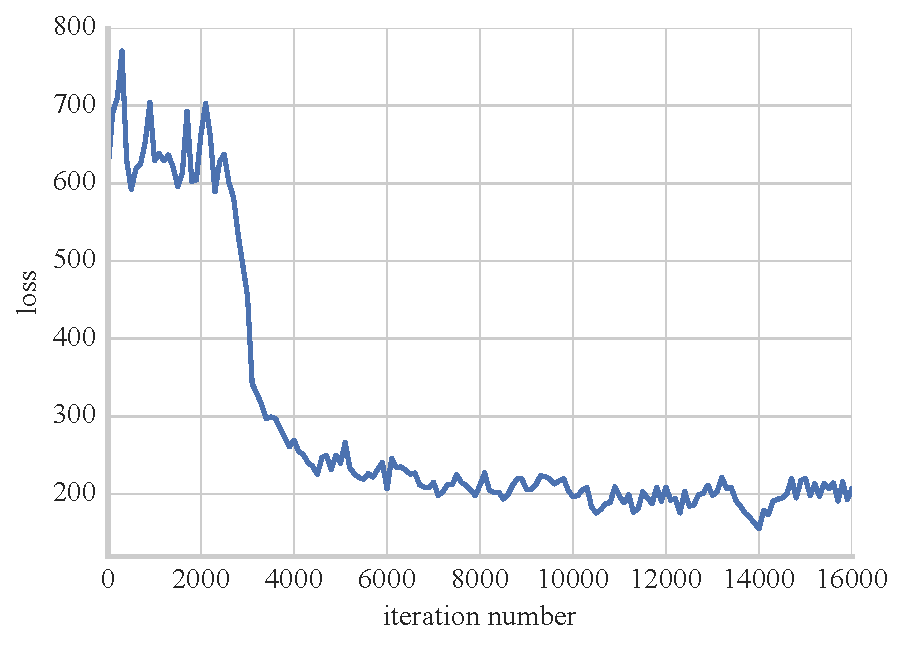
\includegraphics[width=0.8\columnwidth]{figure/obstacle_figs/loss_decrease}
      \caption{The loss decreasing curve as the training iterates. There is a batch of 32 samples used to do back-propagation in every iteration.}
      \label{fig:training_loss}
   \end{figure}
%----------------------------------------------------

Fig.~\ref{fig:training_loss} presents the loss reduction along training iterations. At each iteration, a batch including 32 depth images is randomly chosen from the replay memory. Unlike the training of conventional supervised learning methods, the loss of deep reinforcement learning may not converge to zero, depending extremely on the declaration of the negative reward. Among the estimation Q-values for state-action pairs, the maximum represents the optimal action. The value itself can limited present the sum of the future gains \cite{mnih2015human}. As seen in the figure, the loss converges after 4000 iterations. Test results of several trained models after 4000 iterations are compared in Section \ref{sec:analysis}.

\subsection{Analysis of Policy Tests} \label{sec:analysis}

%-----

We firstly look at the obstacle avoidance capability of the trained model. The trained DRL models after 500, 4000, 7500, and 40000 iterations are chosen to be tested in the simulated environment. The trained supervised learning (SL) model from \cite{tai2016deep} and the reinforcement learning (RL) model from \cite{tl_rcar_2016} are compared directly, without any revision of the model structure or tuning for the weights. In all 12 start points shown in Fig.~\ref{fig:ob_environment_figure}, every model starts ten episodes with the test speeds listed in Table~\ref{tab:moving_commands} for the five moving commands. Additionally, every test episode will stop automatically after 200 moving steps, so that the robot will not explore freely forever. With the same CNN structure for all the trained models, the forward prediction takes $48(\pm5)ms$ for each raw depth input.
After the forward calculation of the received real-time depth image, the robot chooses the moving command with the highest evaluation. The average counts of the moving steps for each start point are listed in Table~\ref{tab:table_heatmapscore}. The more moving steps, the longer the time the robot has been freely moving in the simulated environment without collision.
%---------------------------heatmap-----------------
\begin{figure*}[!ht]
    \centering
    \begin{subfigure}[t]{0.48\columnwidth}
      \centering
      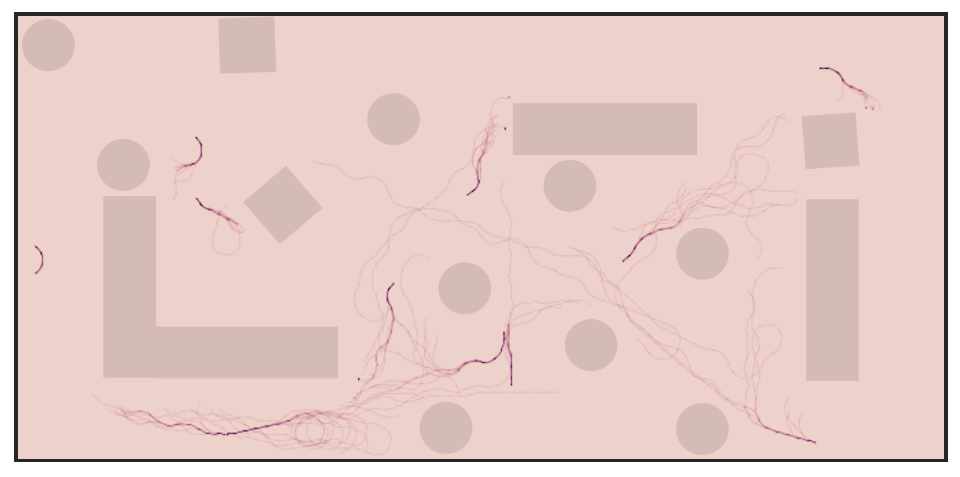
\includegraphics[width=\columnwidth]{obstacle_figs/locateheat/sl}
      \caption{Supervised Learning}
      \label{fig:heatsl}
    \end{subfigure}
    \begin{subfigure}[t]{0.48\columnwidth}
      \centering
      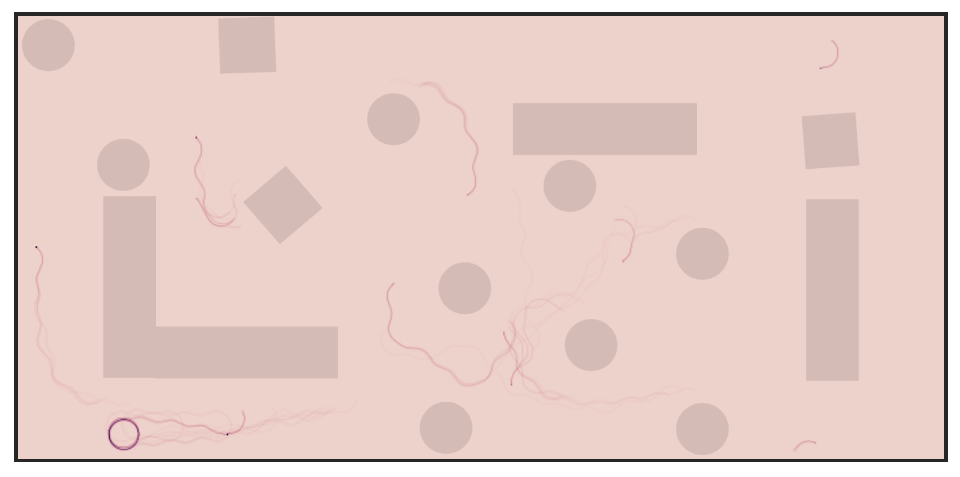
\includegraphics[width=\columnwidth]{obstacle_figs/locateheat/ql}
      \caption{Reinforcment Learning}
      \label{fig:heatql}
    \end{subfigure}
    \begin{subfigure}[t]{0.48\columnwidth}
      \centering
      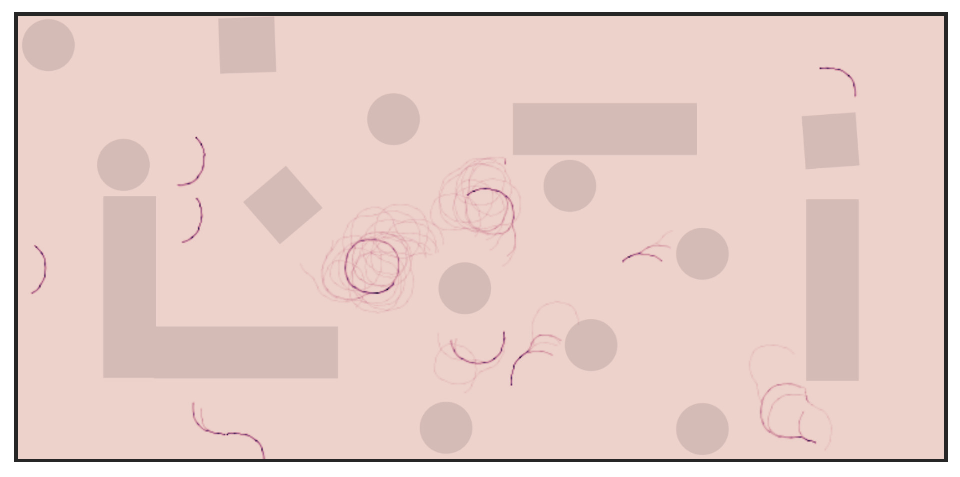
\includegraphics[width=\columnwidth]{obstacle_figs/locateheat/500}
      \caption{DRL 500 iterations}
      \label{fig:heat500}
    \end{subfigure}
    \begin{subfigure}[t]{0.48\columnwidth}
      \centering
      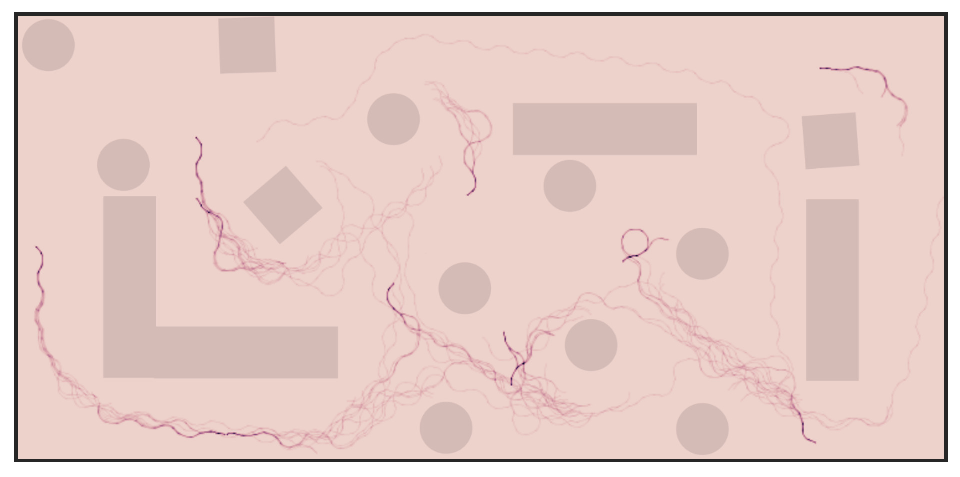
\includegraphics[width=\columnwidth]{obstacle_figs/locateheat/4000}
      \caption{DRL 4000 iterations}
      \label{fig:heat4000}
    \end{subfigure}
    \begin{subfigure}[t]{0.48\columnwidth}
      \centering
      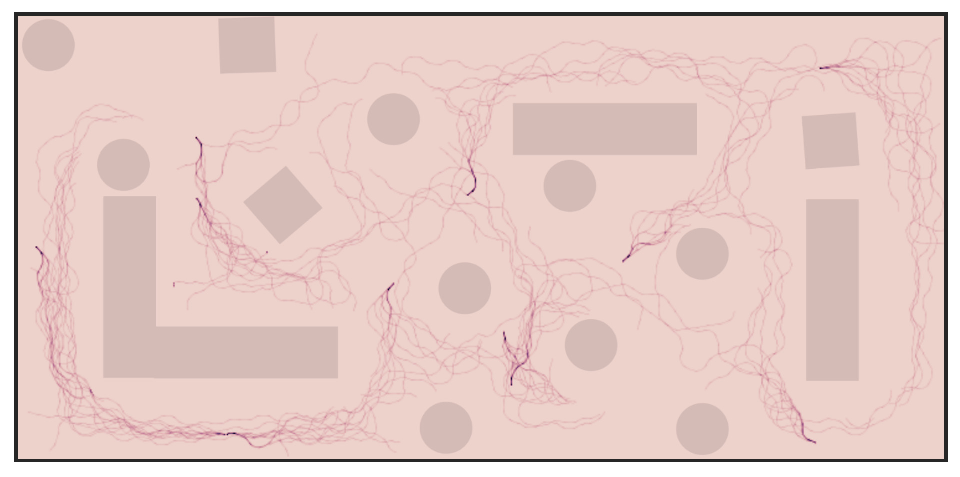
\includegraphics[width=\columnwidth]{obstacle_figs/locateheat/7500}
      \caption{DRL 7500 iterations}
      \label{fig:heat7500}
    \end{subfigure}
    \begin{subfigure}[t]{0.48\columnwidth}
      \centering
      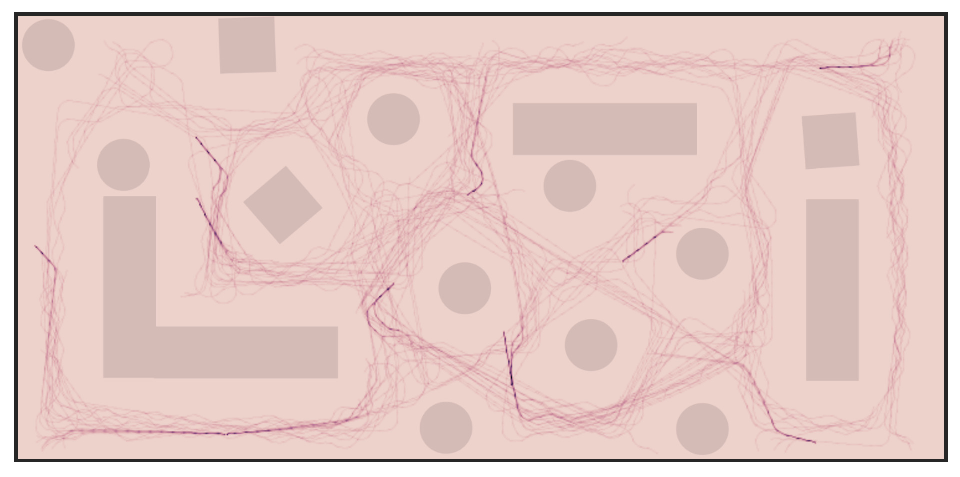
\includegraphics[width=\columnwidth]{obstacle_figs/locateheat/40000}
      \caption{DRL 40000 iterations}
      \label{fig:heat40000}
    \end{subfigure}
    \caption{Heatmaps of the trajectory points' locations in the 10 test episodes of each model for all 12 start points. The counts of points in every map grid are normalized to [0,1]. Note that the circles at the left-bottom corner of (b) and the middle of (c) are actually a stack of circular trajectories caused by the actual motion of the robot.}
    \label{fig:heat_map}
\end{figure*}
%---------------------------------------------------

The moving trajectory points of each model starting from all 12 positions are recorded. Fig.~\ref{fig:heat_map} depicts the trajectory after normalizing the counts of the trajectory points to $[0,1]$ in each map grid of the training environment. The trained model may choose the \textit{left} or \textit{right} command to rotate the robot in place so that no collisions will happen, as depicted in the circles in the left-bottom corner of Fig.~\ref{fig:heatql} and the middle of Fig.~\ref{fig:heat500}, for example. The very large moving count of the RL model in column 2 of Table~\ref{tab:table_heatmapscore} corresponds to the trajectory circle in Fig.~\ref{fig:heatql}. To avoid the appearance of this local minimum, the distances between the start and the endpoint are recorded as an additional evaluation metric. Note that, after a long exploration time, the robot may move back to the area near the start point. So the distance may not be perfectly equal to the obstacle avoidance ability of the trained model.

From the heat maps in Fig.~\ref{fig:heat_map}, we can see that the SL model cannot be adapted to the simulated environment, especially in the scenes with multiple obstacles at different depths and the RL model gives the worst of the results. In the training of the RL model \cite{tl_rcar_2016}, only the weights of the fully-connected network for policy iterations were updated iteratively. The DRL model shows significant improvement compared with the RL model because its training is end-to-end. Thus, not only is the policy network (\textit{fc} layers in Fig.~\ref{fig:network_structure}) developed for complicated scenes, but also the CNN model for feature representations.


Seen in Fig.~\ref{fig:heat_map}(c-f), the training for the obstacle avoidance ability of the DRL model is an online-learning process. In the 500-iteration case, the robot always chooses the same moving direction for any scenes. After 4000 iterations, it can be adapted to parts of the environment. However, In the 7500-iteration case, the robot can almost move freely in the whole simulated world. Furthermore, the robot usually chooses the optimal moving direction after 40000 iterations, like the more efficient trajectories in Fig.~\ref{fig:heat40000}. Unlike the fixed training datasets of the RL model, newly collected training samples of the DRL model are saved to replay memory increasingly. The evaluations of the training scenes are calculated by the current model, which is updated with the increasing number of training iterations. Thus, the robot obstacle avoidance ability will be increased over time.

The 40000-iteration case can almost thoroughly explore the trained environment. Considering the very long training time(12 hours) for 40000 iterations, we choose the model after 7500 iterations to do further analysis. The training time for 7500 iterations is 2.5 hours. This confirms that the mobile robot can be adapted to an unfamiliar environment by transferring the weights of the pre-trained SL model to the DRL framework with very short-term and end-to-end DRL training.

\subsection{Analysis of Receptive Fields in the Cognitive Process}

CNN models are usually considered to be black boxes and the internal activation mechanism of CNN is rarely analyzed. In \cite{zeiler2014visualizing}, the strongest activation areas of the feature representations are presented by backtracking the receptive field in the source input. We propose a backtracking method by multiplying the last layer of feature representations (\textit{pool3} in Fig.~\ref{fig:network_structure}) with a single channel convolutional filter.  The dimension of \textit{pool3} is $64 \times 20 \times 15 $ in this chapter. We multiply it with a convolutional kernel of size $1 \times 15 \times 15$, which is fixed with bilinear weights like the one used for upsampling of semantic segmentation in \cite{long2015fully}. After that, a $120 \times 160$ matrix of the same size as the input images.

\begin{table}[!ht]
    \centering
    \caption{Evaluations of moving commands for different scenes.}
    \label{tab:table_score}
    \begin{tabular}{ c c c c c c c c c}
    \hline
    \hline
      & & & & Left & H-Left & Straight & H-Right & Right \\
    \hline
     \multirow{2}{*}{S1} & & SL&  &$ 23.9 $ &$ \mathbf{26.3} $ &$ -10.6 $ &$ -35.3 $ &$ -34.4 $ \\
          &  &DRL& &$ \mathbf{-16.3} $ &$ -36.2 $ &$ -31.7 $ &$ -38.7 $ &$ -44.5 $ \\
    \hline
     \multirow{2}{*}{S2} & & SL &  &$ -18.2 $ &$ \mathbf{-0.1} $ &$ 46.2 $ &$ -30.1 $ &$ -8.8 $ \\
                 & &DRL& &$ -30.0 $ &$ -25.4 $ &$ -19.8 $ &$ -21.2 $ &$ \mathbf{-15.3} $\\
       \hline
    \multirow{2}{*}{S3} &  &SL&  &$ 4.2 $ &$ 5.9 $ &$ -21.3 $ &$ \mathbf{7.7} $ &$ -0.2 $ \\
                & &DRL& &$ \mathbf{-5.3} $ &$ -15.3 $ &$ -13.0 $ &$ -16.5 $ &$ -19.9 $ \\
       \hline
         \multirow{2}{*}{S4} & &SL&  &$ -4.0 $ &$ -5.5 $ &$ -15.2 $ &$ \mathbf{13.3} $ &$ -0.4 $ \\
                & &DRL& &$ -4.6 $ &$ -5.1 $ &$ \mathbf{-3.8} $ &$ -4.8 $ &$ -4.3 $ \\
     \hline
     \multirow{2}{*}{S5} & &SL&  &$ -17.4 $ &$ 12.3 $ &$ \mathbf{23.0} $ &$ -9.7 $ &$ -18.4 $ \\
            & &DRL& &$ \mathbf{-9.9} $ &$ -19.2 $ &$ -15.8 $ &$ -19.2 $ &$ -21.6 $ \\
    \hline
       \hline
     \multirow{2}{*}{R1} & &SL&  &$ -38.2 $ &$ 17.5 $ &$ \mathbf{27.4} $ &$ -15.6 $ &$ -1.9 $ \\
            & &DRL& &$ -84.1 $ &$ -89.3 $ &$ -71.8 $ &$ -78.8 $ &$ \mathbf{-63.2} $ \\
    \hline
     \multirow{2}{*}{R2} & &SL&  &$ -11.6 $ &$ \mathbf{45.6} $ &$ -50.3 $ &$ 4.1 $ &$ -8.3 $ \\
        & &DRL& &$ -8.3 $ &$ -9.3 $ &$ \mathbf{-7.1} $ &$ -8.6 $ &$ -7.5 $ \\
    \hline
     \multirow{2}{*}{R3} & & SL& &$ -18.4 $ &$ 32.2 $ &$ \mathbf{37.2} $ &$ -23.3 $ &$ -41.4 $ \\
        & &DRL& &$ \mathbf{-87.7} $ &$ -113.3 $ &$ -90.9 $ &$ -103.6 $ &$ -96.3 $ \\
       \hline
         \multirow{2}{*}{R4} & &SL& &$ 4.2 $ &$ 1.1 $ &$ -7.8 $ &$ -10.1 $ &$ \mathbf{15.2} $ \\
        & &DRL& &$ \mathbf{-87.6} $ &$ -141.1 $ &$ -115.2 $ &$ -134.8 $ &$ -137.4 $ \\
       \hline
         \multirow{2}{*}{R5}& &SL&  &$ 0.4 $ &$ -6.2 $ &$ -48.8 $ &$ \mathbf{32.8} $ &$ 11.9 $ \\
        & &DRL&    &$ -3.4 $ &$ -3.3 $ &$ \mathbf{-2.5} $ &$ -3.0 $ &$ -2.7 $ \\
    \hline
    \end{tabular}
\end{table}
%-------------------------------------------------------------------------------------------------

%-------------receptive real figure---------------------
\begin{figure*}[!ht]
    \centering
    \begin{subfigure}[t]{0.48\columnwidth}
      \centering
      \includegraphics[width=\columnwidth]{obstacle_figs/receptive/simurecpt}
      \caption{Simulation environmental samples}
      \label{fig:recep_simu}
    \end{subfigure}
    \begin{subfigure}[t]{0.48\columnwidth}
      \centering
      \includegraphics[width=\columnwidth]{obstacle_figs/receptive/simurecpt}
      \caption{Real-world samples}
      \label{fig:recep_real}
    \end{subfigure}
    \caption{The receptive fields of the feature representations extracted by CNN in both simulated environment samples and real-world samples. The purple area marked on the raw depth image represents the highest $10\%$ of activation values. Both the supervised learning model (SL) and the 7500-iteration deep reinforcement learning model (DRL) are compared. The arrow at the bottom of each receptive image is the chosen moving command based on evaluations listed in Table.~\ref{tab:table_score}. The left column shows the RGB images taken from the same scenes, for reference.}
    \label{fig:recep}
\end{figure*}
%----------------------------------------------------

We focus on the most substantial activation area of the receptive matrix. Fig.~\ref{fig:recep_simu} shows the highest $10\%$ of values of this matrix, marked on the related raw depth images in five specific simulated training samples. The receptive fields of the 7500-iteration DRL model are compared with those extracted from the SL model \cite{tai2016deep}. As mentioned above, these two models consist of the same convolutional structures. We choose five specific samples located in the fallible area based on the trajectory heat map of the SL model, as shown in Fig.~\ref{fig:heatsl}. Before being transported to the \textit{Softmax} layer, feature representations of the SL model were firstly transformed to five values related to the five commands in \cite{tai2016deep}. These values are listed with the action-evaluations estimated by the 7500-iteration DRL model in Table~\ref{tab:table_score}. For both of the models, the highest value corresponds to the optimal moving command.

%especially the untracked part
Note that the area beyond the detection range of the \textit{Kinect} camera is labelled as zero in the raw depth images. From Fig.~\ref{fig:recep_simu} and Table~\ref{tab:table_score}, for the SL model, the moving command towards the deepest area in the range receives the highest output value naturally. This motivates the convolutional model to activate the further area of the scenes, especially the junction with the untracked white fields. In \textit{S1}, the furthest reflection can help the robot avoid close obstacles. However, when there are multiple-level obstacles like in \textit{S2} and \textit{S3}, simply choosing the furthest part as the moving direction leads to collisions with nearby obstacles. Except for the furthest part, the DRL model also perceives the width of the route, both in the nearby area and the furthest area, as several horizontal cognitive stripes in the figure. That means the end-to-end deep reinforcement learning dramatically tunes the initial CNN weights from the SL model. From evaluations listed in Table~\ref{tab:table_score}, the DRL model not only helps the robot avoid instant obstacles, but also improves the traversable detection ability, like in \textit{S4} and \textit{S5}.
When the route in \textit{S4} is not wide enough to pass through, the DRL model chooses the fully turning moving command. However, the SL model always chooses the furthest area.

To prove the robustness of the trained model, five samples collected from a real-world environment by a \textit{Kinect} camera mounted on a real \textit{Turtlebot} are also tested, as shown in Fig.~\ref{fig:recep_real}. The related command evaluations for the SL model and the DRL model, as mentioned above, are listed in Table~\ref{tab:table_score} as well. Note that, these real-world scenes are not included in the training datasets for the SL model \cite{tai2016deep} either. The receptive fields of the SL model are still mainly focused on the furthest area. Output values in Table~\ref{tab:table_score} present the limited obstacle avoidance ability of the SL model for theses untrained samples. For the DRL model, even though only trained in the simulated environment, it keeps showing its ability to track the width of the route for real-world samples. In \textit{R1} and \textit{R2}, the trained DRL model successfully detects the traversable direction.
In \textit{R3}, it avoids the narrow space which is not wide enough to pass through. In \textit{R4}, it chooses the optimal moving direction to turn fully left. However, in \textit{R5}, when faced with irregular nearby obstacles which are not implemented in the training environment, it keeps tracking the width of the furthest area and fails to avoid irregular obstacles.

Another fact about the real-world tests is that the estimation of the action-value can reflect the future expectation to some extent. The estimation values of \textit{R3} and \textit{R4} listed in Table.~\ref{tab:table_score} for all moving commands are obviously less than the values of other scenes. This corresponds to the higher probability of collision when there are nearby obstacles.
